% !TEX root = ../thesis.tex
% adjust parameter limits
% @author Tobias Wulf
%

\section{Anpassung der Parametergrenzen}\label{sec:exp4}

\textbf{Zweck:} Das Experiment besitzt einen veranschaulichenden Charakter und soll zeigen, wie der Rechenaufwand für die Optimierungen nach \autoref{alg:fminconopt} und \autoref{alg:bayesopt} verringert werden kann. Dafür werden die Parameter der Kovarianzfunktion in Abhängigkeit der Modellplausibilitäten nach \autoref{eq:fmincon} untersucht und das Rauschniveau in Verbindung mit den mittleren Modellverlust $MSLL$ nach \autoref{eq:bayesopt} gezeigt. Ziel ist es, die Durchlaufzahl für die äußere Optimierung über das Rauschniveau und \autoref{alg:bayesopt} zu verkürzen und dabei die Generalisierung des Modells aufrechtzuerhalten.
Aussagen zur Modellgeneralisierung und Modellanpassung auf den Trainingsdaten sind den Anhängen \autoref{sec:gpropt} und \autoref{sec:gprgen} zu entnehmen.

\textbf{Durchführung:} Das Experiment wir in zwei Durchgängen durchgeführt. In beiden wird Regressionsmodell nach \autoref{eq:de2innorm} und \autoref{eq:kfun} mittels \autoref{alg:fminconopt} und \autoref{alg:fminconopt} optimiert und anschließend ein Parameter-Sweep für die Parameter der Kovarianzfunktion in Abhängigkeit der Modellplausibilität nach \autoref{eq:fmincon} durchgeführt. Der Parameter-Sweep wird für jeden Parameter für eine zusätzliche Dekade neben den Parametergrenzen ausgeführt. Der erste Durchgang wird mit der Default-Konfiguration aus \autoref{tab:sim-params-exp} ausgeführt. Danach werden die Parametergrenzen angepasst, die Durchlaufzahl verringert und das Experiment wiederholt.

\textbf{Erzeugte Datensätze:} Jeweils ein Trainings- und Testdatensatz mit korrespondierender Position des Sensors und Verkippungswinkel des Magneten.

\textbf{Matlab-Skript:} investigateKernelParameters.m, siehe \autoref{mcode:investigatekernelparameters}

\textbf{Abweichende Parameter von \autoref{tab:sim-params-exp}:}


\vspace{5mm}
\begin{table}[htp]
	\centering
	\resizebox{\textwidth}{!}{
		\begin{tabular}{l l c l}
			\toprule
			\textbf{Parametergruppe} & \textbf{Parameter}  & \textbf{Wert}        & \textbf{Kurzbeschreibung}                          \\ \midrule
			TrainingOptions          & nAngles             & $17$                 & Simulationswinkelanzahl angepasst                  \\ \hline
			GPROptions               & kernel              & 'QFCAPX'             & Indikator für zweite Kernel-Variante               \\
			                         & $\sigma_f^2$-Bounds & $(1, 10)$            & Parameter-Bounds $\theta_1 = \sigma_f^2$ angepasst \\
			                         & $\sigma_l$-Bounds   & $(10, 30)$           & Parameter-Bounds $\theta_2 = \sigma_l$ angepasst   \\
			                         & $\sigma_n^2$-Bounds & $(10^{-6}, 10^{-4})$ & Parameter-Bounds $\sigma_n^2$ angepasst            \\
			                         & OptimRuns           & $10$                 & Durchlaufanzahl äußere Optimierung verringert      \\
			                         & mean                & 'zero'               & Mittelwertpolynom ausgeschaltet                    \\ \bottomrule
		\end{tabular}}
	\caption{Abweichende Simulationsparameter im Experiment zur Parametergrenzenanpassung.}
	\label{tab:params-exp4}
\end{table}


\clearpage


\textbf{Ergebnisse:} Die Ergebnisse des Durchgangs sind grafisch in \autoref{fig:qfcapx-z-n17-bounds} und \autoref{fig:qfcapx-z-n17-opt} ausgewertet. \autoref{fig:qfcapx-z-n17-bounds} zeigt die Anpassung der Parametergrenzen für die Optimierungsalgorithmen und \autoref{fig:qfcapx-z-n17-opt} veranschaulicht die Verringerung der Durchlaufzahl für die äußere Optimierung.



\textbf{Beobachtungen:} Die engeren Parametergrenzen für die Parameter der Kovarianzfunktion stecken ein engeres Suchfeld für das innere Minimierungsproblem ab, zu sehen in \autoref{fig:qfcapx-z-n17-bounds} b). Der Algorithmus findet das Minimum und besitzt noch genügend Freiraum, sodass die Parametergrenzen nicht verletzt werden. In Teil a) der \autoref{fig:qfcapx-z-n17-bounds} schafft es die äußere Optimierung den Schwellwert für die Generalisierung entsprechend gut abzusenken. Es gibt ebenfalls keine Verletzungen der Parametergrenzen. Das Minimum ist extrem und Fehlergrenzen des Algorithmus können nach wenigen Schritten im Bereich des Minimums stark eingegrenzt werden. Die \autoref{fig:qfcapx-z-n17-opt} beobachtet die Minimum-Kriterien der Algorithmen in Bezug auf die Anzahl der Durchläufe. Abbildung a) für die äußere Optimierung und b) sowie c) für die innere Optimierung. Die innere Optimierung wird bei jedem Durchlauf der äußeren wiederholt, siehe \autoref{sub:gpr-pro}. Zu sehen ist der letzte Durchlauf der inneren Optimierung in b) und c). Die äußere Optimierung schafft es nach acht Durchläufen einen stabilen Wert für die Generalisierung zu erreichen. Im letzten Durchgang der inneren Optimierung sind die optimalen Parameter nach fünf Durchgängen gefunden. Die Innere Optimierung benötigt eine gewisse Durchlaufzahl um festzustellen, dass keine markanten Änderungen geschehen und das Minimum gefunden ist. Die äußere Optimierung benötigt die Begrenzung über die Durchlaufzahl.


\clearpage
\begin{figure}[tph]
	\centering
	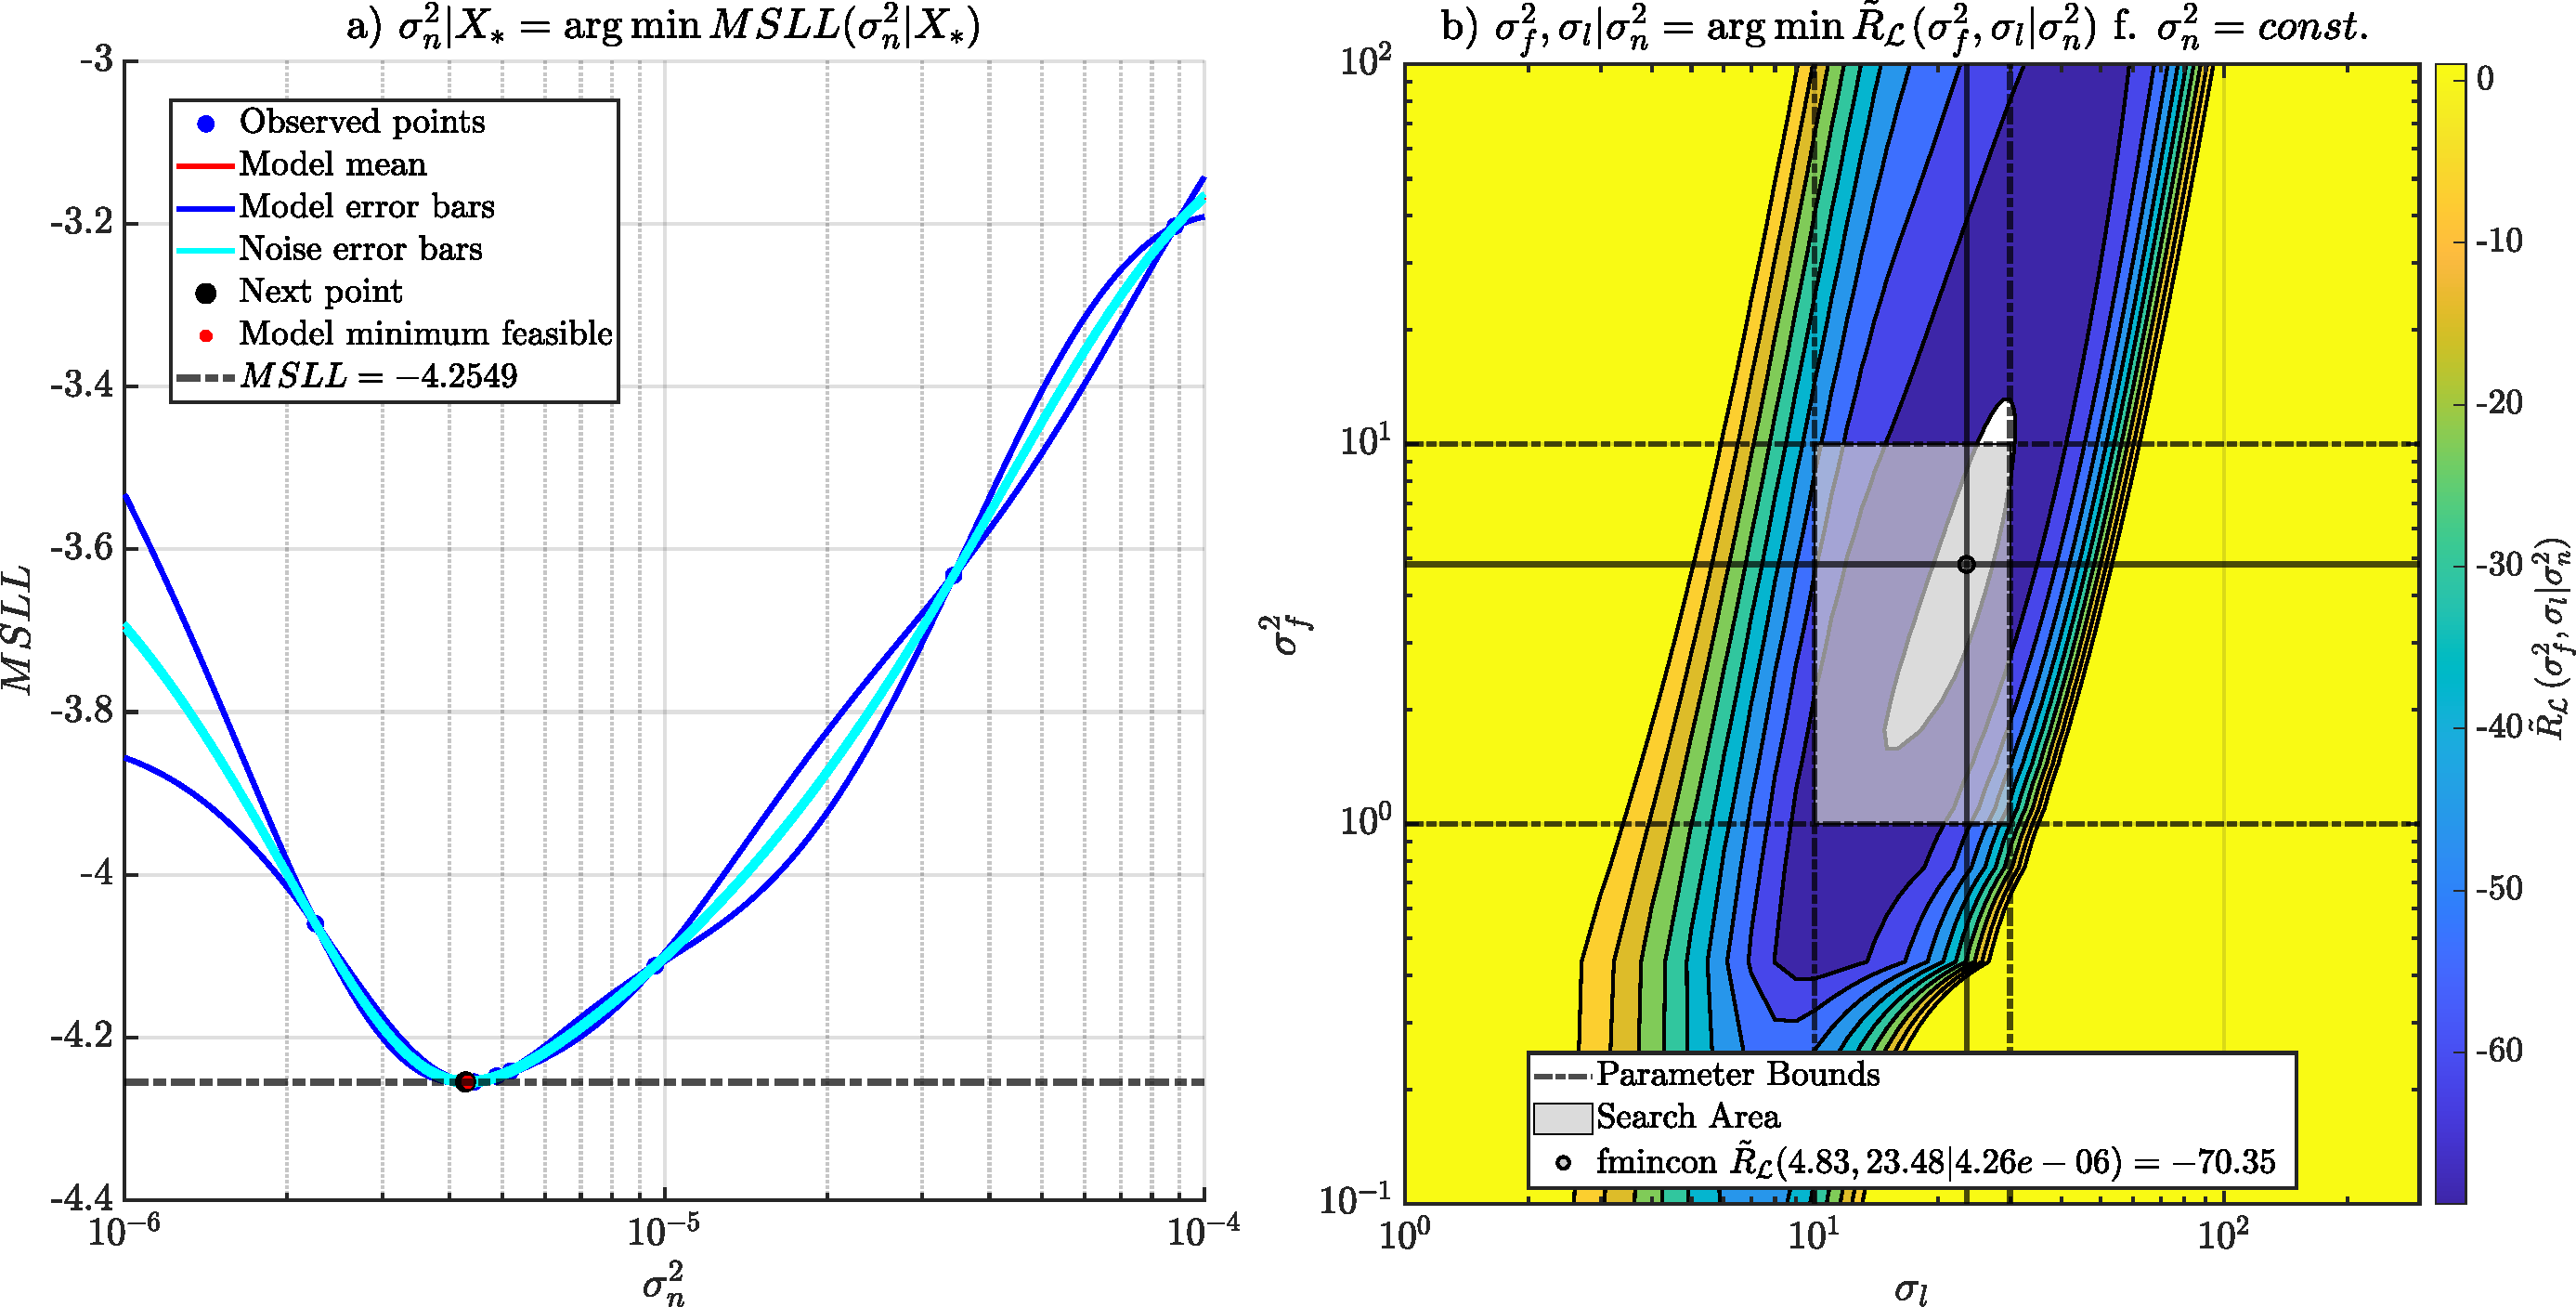
\includegraphics[width=\linewidth]{chapters/images/4-EuOExp/QFCAPX-Z-N17-Bounds}
	\caption[Äußere und innere Modelloptimierung mit angepassten Parametergrenzen]{Äußere und innere Modelloptimierung mit angepassten Parametergrenzen. Die äußere Modelloptimierung in a) für das Rauschniveau $\sigma_n^2$ nach \autoref{alg:bayesopt} und \autoref{eq:bayesopt}. Der mittlere standardisierte logarithmische Verlust $MSLL$ (engl. Loss) ist für alle eingespeisten Testdaten $X_*$ in a) berechnet und ist das Schwellwertkriterium für die Modellgeneralisierung. Die äußere Optimierung gibt das Rauschniveau $\sigma_n^2$ für die innere Optimierung in b) vor. In b) werden basierend auf den eingespeisten Trainingsdaten die Parameter der Kovarianzfunktion nach \autoref{alg:fminconopt} und \autoref{eq:fmincon} getrimmt. Die Optimierung stützt sich auf die Summe der logarithmischen Plausibilitäten (engl. Log. Marginal Likelihoods) für die zu vorhersagenden Cosinus- und Sinus-Funktionen. Beide Optimierungen suchen nach einem Minimum. Hier gezeigt mit angepassten Parametergrenzen in a) für $\sigma_n^2 = (10^{-6}, 10^{-4})$ und in b) für $\sigma_f^2 = (1, 10)$ und $\sigma_l = (10, 30)$. Grafik nachempfunden aus \cite{Rasmussen2006}.}
	\label{fig:qfcapx-z-n17-bounds}
\end{figure}



\clearpage
\begin{figure}[tph]
	\centering
	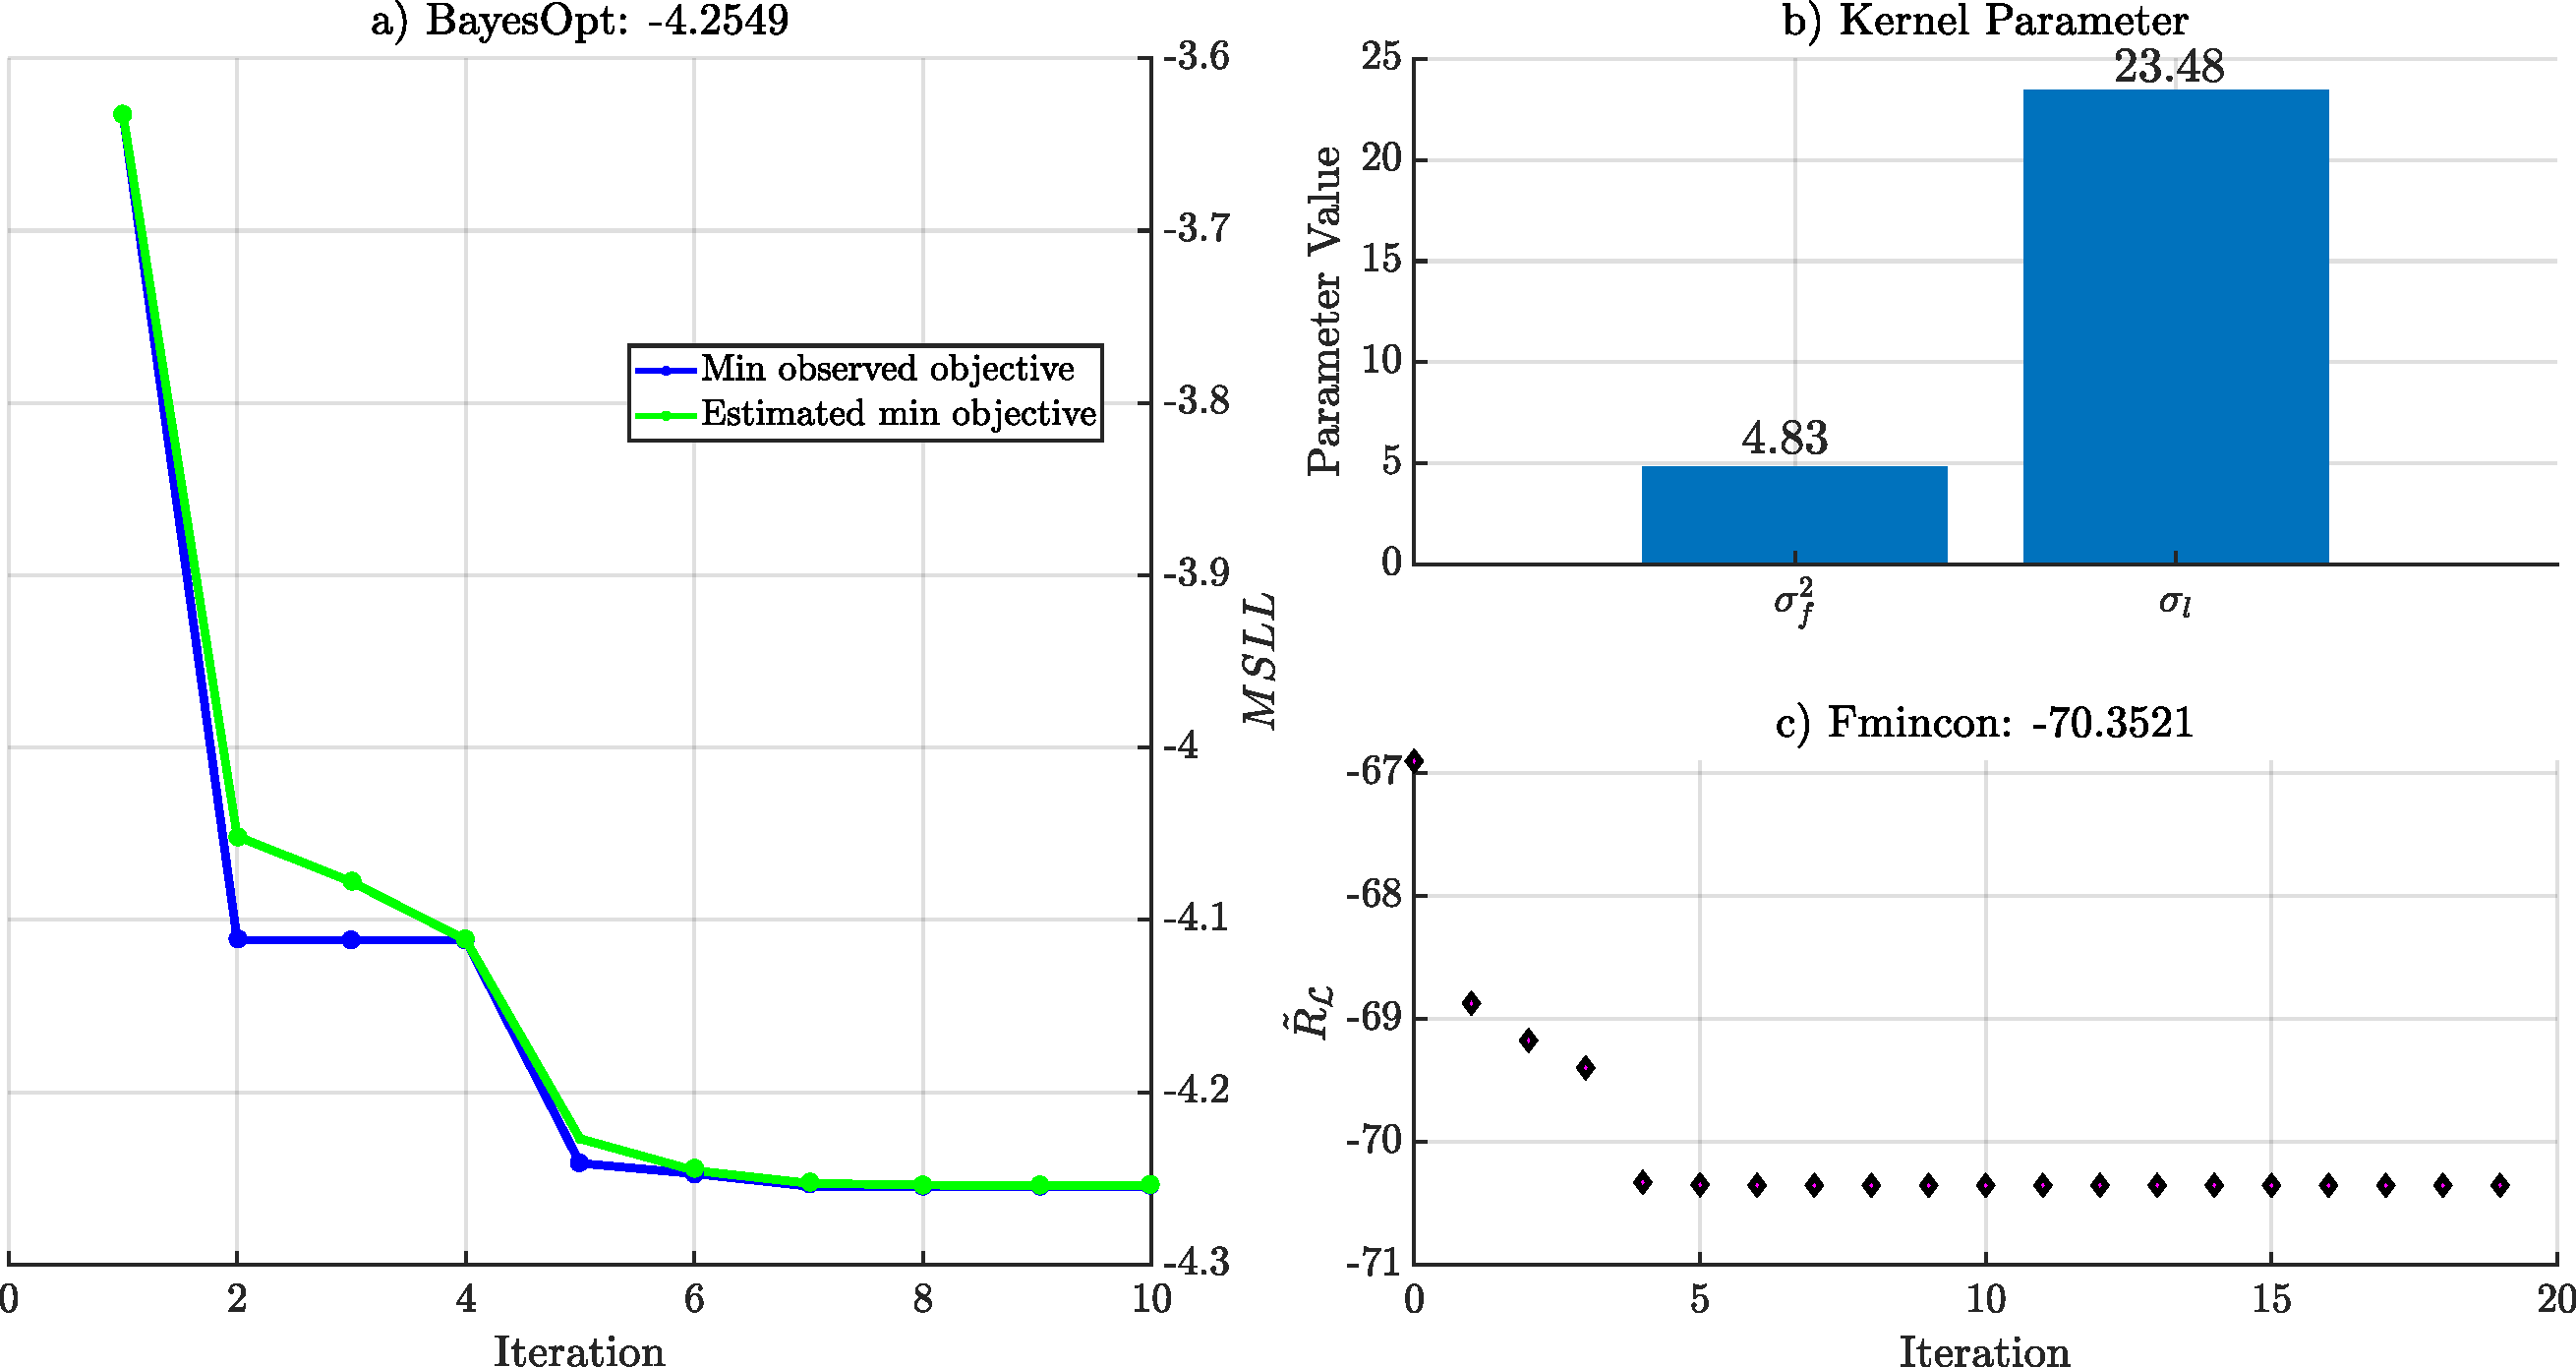
\includegraphics[width=\linewidth]{chapters/images/4-EuOExp/QFCAPX-Z-N17-Opt}
	\caption[Äußere und innere Modelloptimierung mit angepasster Durchlaufzahl]{Äußere und innere Modelloptimierung mit angepasster Durchlaufzahl. Nach Anpassung der Parametergrenzen in \autoref{fig:qfcapx-z-n17-bounds}, ist die Durchlaufzahl für die äußere Modelloptimierung nach \autoref{alg:bayesopt} von $30$ auf $10$ Durchläufe verringert worden. Es gelingt in a) nach $10$ ein stabile Generalisierung mit negativen mittlerem standardisierten logarithmischen Verlust (engl. Loss) $MSLL$ zu finden. Die innere Optimierung in b) und c) nach \autoref{alg:fminconopt} bedarf vorerst keine weiterer Anpassung. Diese ist relativ zur äußeren Optimierung sehr viel schneller, da sie nur mit Trainingsdaten arbeitet.}
	\label{fig:qfcapx-z-n17-opt}
\end{figure}


\clearpage

